\documentclass[10pt, conference, compsocconf, onecolumn]{IEEEtran}
\IEEEoverridecommandlockouts
\usepackage{amsmath}
\usepackage{amssymb}
\usepackage{amsthm}
\usepackage{lipsum}
\usepackage[justification=centering,font=footnotesize, labelfont=bf]{caption}
\usepackage{listings}
\usepackage{gensymb}
\usepackage{fancyhdr}
\usepackage{graphicx}
\usepackage{algorithm}
\usepackage{algpseudocode}
\usepackage{subcaption}
\usepackage{mwe}
\newtheorem{thma}{Theorem}
\newtheorem{prop}{Proposition}
\newtheorem{lemm}{Lemma}
\usepackage{svg}

% correct bad hyphenation here
\hyphenation{op-tical net-works semi-conduc-tor}

% commands


\begin{document}
%
% paper title
% can use linebreaks \\ within to get better formatting as desired
\title{Aplicaci\'on de \textit{Paralelismo Din\'amico} para el
	mapeo eficiente de threads de GPU en problemas de
	dominio tetra\'edrico\\}


% author names and affiliations
% use a multiple column layout for up to two different
% affiliations

\author{
\IEEEauthorblockN{Gabriel A. Gonz\'alez}
\IEEEauthorblockA{Instituto de Inform\'atica,\\
Universidad Austral de Chile,\\
Valdivia, Chile\\
Email: gabriel.gonzalez.uribe@alumnos.uach.cl}
}

% make the title area
\maketitle


\begin{abstract}
% Al momento de mapear threads de ejecución en programación en GPU, hay threads que bajo ciertas situaciones como problemas de dominio triangular, son descartados en tiempo de ejecución. Esto es un problema, ya que vuelve la programación en GPU ineficiente en cuanto a tiempo de ejecución desperdiciado y espacio en threads de ejecuci\'on. El trabajo que se presenta a continuación, estudia el paralelismo dinámico aplicado a una superficie cubica en R3 donde se descartarán aquellos threads de ejecución que están por sobre el plano diagonal de un cubo \textit{($x+y > z$)}. Primero se estudia el caso donde el mapeo se realiza utilizando paralelismo dinámico, donde se generan bloques de threads de ejecución de forma recursiva. Frente a un método trivial donde simplemente se descartan aquellos threads que no se ocuparan y que están por sobre la superficie diagonal en tiempo de ejecución. Una vez comparados ambos m\'etodos se logr\'o concluir que el paralelismo din\'amico tiene una notable mejora de hasta casi 4x en GPU con arquitectura VOLTA.
 
  In GPU computing there is a stage in the execution pipeline where threads are mapped to the data domain. Under certain situations such as triangular domain problems, the traditional programming  would generate threads that will be discarded at runtime. This is a problem, since it makes the programming in GPU inefficient in terms of wasted execution time and space in execution threads. The main purpose of this article is to study the \textit{dynamic parallelism} feature applied to tetrahedral domain problems. First, we study the case where the mapping is performed using dynamic parallelism, i.e. blocks of execution threads are recursively generated. Then, we consider the brute force method where threads are discarded at runtime. Based on the results, we concluded that the dynamic parallelism approach did not offer any speedup for Kepler and Pascal GPU architectures, but for Volta it offered  a remarkable improvement of up to $\sim 3\times$. The results obtained in this article make the mapping through Dynamic Parallelism an alternative to be considered in Volta GPUs for the solution of tetrahedral domain problems.
\end{abstract}

\begin{IEEEkeywords}
GPU computing; Dynamic Parallelism; Mapping threads ;
\end{IEEEkeywords}


% For peer review papers, you can put extra information on the cover
% page as needed:
% \ifCLASSOPTIONpeerreview
% \begin{center} \bfseries EDICS Category: 3-BBND \end{center}
% \fi
%
% For peerreview papers, this IEEEtran command inserts a page break and
% creates the second title. It will be ignored for other modes.
\IEEEpeerreviewmaketitle



\section{Introducci\'on}
\label{sec_introduccion}


La programaci\'on en GPU es un recurso que en este \'ultimo tiempo ha contribuido en el avance de varias \'areas de la inform\'atica. Donde m\'as se destaca este avance es en el \'area de los video juegos, animaci\'on 3D y todo lo que respecta a procesamiento gr\'afico en general. Pero no solo en este aspecto ha contribuido la GPU, sino que tambi\'en en el \'area de la computaci\'on de alto rendimiento (HPC). La raz\'on de este crecimiento es debido a la arquitectura de la GPU, que a diferencia de la CPU que tiene uno o varios n\'ucleos, de gran potencia, la GPU est\'a constituida de muchos n\'ucleos (de un orden de miles o m\'as) por lo que se puede aprovechar bastante el paralelismo masivo en este tipo de arquitectura, logrando, en gran parte de los casos, tiempos de ejecuci\'on significativamente m\'as bajos, que en una CPU convencional. De esta forma la computaci\'on de alto rendimiento puede beneficiar \'areas como la inteligencia artificial, c\'alculos financieros, an\'alisis de datos, investigaciones cient\'ificas, entre otras.

Una de las principales caracter\'isticas que posee el  modelo de computo de las GPUs, es que est\'an dise\~nadas para trabajar con dominios lineales, cuadrados, rectangulares o paralelep\'ipedos en el caso de dominios en tres dimensiones. Al ejecutar un c\'alculo en paralelo, todos los \textit{threads} primero deben agruparse geom\'etricamente como una lista, matriz o paralelep\'ipedo dependiendo si el problema es  1D, 2D o 3D, respectivamente. Idealmente el dominio de datos del problema debiese seguir la misma geometr\'ia que la que contiene los \textit{threads} agrupados. Cuando esto se cumple, la GPU logra utilizar todos sus \textit{threads} de manera eficiente ya que todos estos participan haciendo parte del trabajo necesario. Sin embargo, cuando la geometr\'ia del dominio de datos es distinta a la geometr\'ia que contiene los \textit{threads}, surge un problema de rendimiento, ya que la geometr\'ia que contiene los \textit{threads} no coincidir\'a e inevitablemente existir\'an \textit{threads} innecesarios que ser\'an descartados en tiempo de ejecuci\'on. Un caso que se presenta en algunos problemas de la ciencia y tecnolog\'ia es el de dominio tetra\'edrico. Este problema geom\'etricamente se puede representar como un tetraedro. Para este problema particular surge la siguiente pregunta de investigaci\'on. ?`Pueden las \'ultimas tecnolog\'ias de GPU, tales como \textit{Dynamic Parallelism}, reducir la cantidad de threads para dominios de tetraedro en tres dimensiones y entregar una mejora en rendimiento como consecuencia?


Este trabajo busca estudiar \textit{Dynamic Parallelism} o paralelismo din\'amico en problemas donde el dominio del problema modelado en $\mathcal{R}^3$ puede resultar un tetraedro. Estos problemas se llamar\'an de ahora en adelante \textit{problemas de dominio tetra\'edrico}. Este tipo de problemas pueden existir en \'areas como la f\'isica, qu\'imica y ciencias en general tales como la sistemas din\'amicos, simulaciones y ecuaciones en derivadas parciales (PDEs) \cite{3body2014} \cite{ThreadMapforSimplex2018}. El desaf\'io desde la ciencia de la computaci\'on es buscar formas eficientes para mapear \textit{threads} a espacios de tipo tetraedro.

La problem\'atica presentada en este trabajo es an\'alogo a \textit{td-problem} \cite{TriMap2013} donde se trata el espacio de mapeo en dos dimensiones sobre dominios triangulares en los cuales los \textit{threads} que est\'an por sobre  la l\'inea diagonal (cuando \textit{$x>y$}) se descartan. Algo similar ocurre en tres dimensiones donde los \textit{threads} que est\'an por sobre el plano diagonal $x+y>z$ se descartan. El principal hallazgo de este estudio, es que no existe una mejora notable en la eficiencia al utilizar \textit{dynamic parallelism} excepto para el caso  en que se usa la GPU Tesla V100 donde se encontr\'o una mejora de hasta  $\sim 3\times$ en comparaci\'on al m\'etodo fuerza bruta.

El art\'iculo se encuentra estructurado, para un mejor entendimiento, comenzando por la secci\'on ``Modelo De Programaci\'on", donde se explican algunos conceptos para entender el art\'iculo, como CUDA, \textit{dynamic parallelism} y problemas de dominio tetra\'edrico. Luego sigue la secci\'on ``Trabajos Relacionados", donde se contextualizar\'a este trabajo describiendo brevemente algunos trabajos relacionados a este. La secci\'on ``Soluci\'on Propuesta", explica con detalle el desarrollo de la soluci\'on propuesta. En ``Resultados de Rendimiento", se da a conocer el resultado de este algoritmo recursivo probado en cuatro distintas m\'aquinas y comparando este algoritmo con una t\'ecnica m\'as convencional. En ``Discusi\'on" se analizan los gr\'aficos con m\'as detalle y se plantean posibles trabajos futuros sobre los resultados arrojados en este estudio. Finalmente, en la secci\'on ``Conclusi\'on" se obtendr\'an conclusiones de este trabajo en general.

\section{Modelo de programaci\'on en GPU}
\label{sub_sec_Mod}

En esta secci\'on se abordan algunos conceptos fundamentales para la soluci\'on propuesta. Se explica el modelo de programaci\'on CUDA, el paradigma utilizado para la resoluci\'on del problema que es \textit{dynamic parallelism} y el concepto de problema de dominio tetra\'edrico.

\subsection{CUDA}
\label{sub_sec_ModCuda}

Para el desarrollo de este estudio se utiliz\'o CUDA, cuya sigla en ingles significa \textit{Compute Unified Device Architecture} \cite{ScalCuda2008}, lenguaje basado en C que funciona mediante una jerarquizaci\'on espacial para distribuir el computo en los n\'ucleos de una GPU. Dentro de la terminolog\'ia b\'asica de CUDA se encuentran los t\'erminos \textit{Host} y \textit{Device}, cuando se menciona el termino \textit{host} se refiere a la CPU. Mientras que el termino \textit{device} se refiere a la GPU. En la GPU  existe una memoria que almacena los datos a utilizar en los c\'alculos de la GPU,  es por esto que existe un tiempo de traspaso de datos entre \textit{device} y \textit{host} que se puede percibir cuando la matriz de datos a tratar es muy grande y el c\'alculo se hace una sola vez, pero que, en este caso, se omite dado a que este tiempo se vuelve imperceptible a medida que la cantidad de computo supera a la cantidad de traspasos entre \textit{host} y \textit{device}.


 
 En CUDA el c\'odigo que se ejecuta y es invocado a trav\'es de otro lenguaje como en este caso es C, se llama \textit{kernel}, en cada \textit{kernel} se puede especificar si el c\'odigo se ejecuta en \textit{host} o \textit{device}. Si el c\'odigo se ejecuta en \textit{device}, cada \textit{kernel} recibe el n\'umero de \textit{threads} en donde se ejecutar\'a, estos \textit{threads} se ejecutan de forma paralela en la GPU, organizados mediante una jerarquizaci\'on espacial. Como se puede ver en la Figura \ref{fig_Jerarquia}, esta jerarquizaci\'on comienza con los \textit{threads} de ejecuci\'on. Luego, le siguen los bloques o \textit{blocks}, donde cada \textit{block} est\'a compuesto por $N$ \textit{threads} de ejecuci\'on \footnote{El tama\~no y la elecci\'on de \textit{block} se explican en secci\'on \ref{ele_blocksize}.}. En el \'ultimo nivel se encuentra lo que se conoce como \textit{grid}, que es la agrupaci\'on de los \textit{blocks} en una malla o grilla. Para ejecutar un \textit{kernel} en la GPU se debe especificar el tama\~no del \textit{block} (n\'umero de \textit{threads} por \textit{block}) y el tama\~no de la grilla o \textit{grid} (n\'umero de \textit{blocks} por \textit{grid}). Cada \textit{thread} tiene un \'indice o identificador dentro del \textit{block} y cada \textit{block}, tiene un \'indice dentro del \textit{grid}.
\begin{figure}[H]
	\centering
	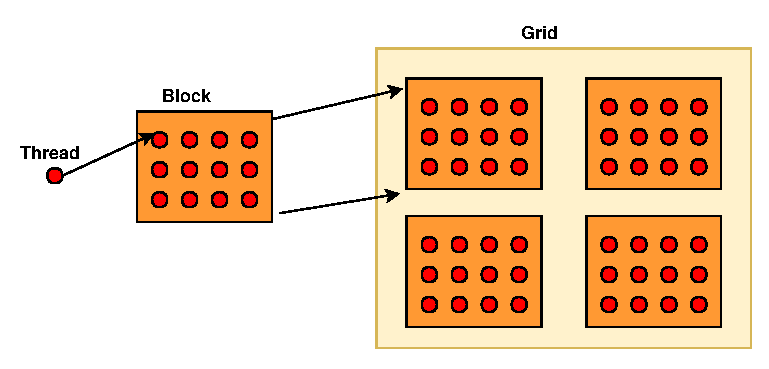
\includegraphics[scale=0.8]{figures/Jerarquia_mem.eps}
	\caption{Representaci\'on de jerarqu\'ia espacial en CUDA}
	\label{fig_Jerarquia}
\end{figure}

\subsection{\textit{Dynamic Parallelism}}
\label{sub_sec_ModPD}



\textit{Dynamic Parallelism} \cite{DinamicParallelism} \cite{TriMap2013}, es una t\'ecnica utilizada en programaci\'on en GPU, que se ha promocionado como una t\'ecnica que extiende el modelo de programaci\'on y a la vez puede mejorar el rendimiento. Sin embargo, esta \'ultima propiedad no se ha podido confirmar claramente en la literatura actual. Esta t\'ecnica consiste en hacer llamadas recursivas de \textit{kernels} de CUDA, donde cada \textit{kernel} ejecuta un cierto n\'umero \textit{threads} de forma paralela en los n\'ucleos de la GPU. Es decir, como se ve en la Figura \ref{fig_Parelismodinamico}, desde un \textit{kernel} en ejecuci\'on con m\'ultiples \textit{threads}, es posible lanzar otro \textit{kernel} de ejecuci\'on que a su vez tambi\'en puede lanzar m\'as \textit{kernels} en ejecuci\'on. Esta t\'ecnica se puede utilizar en los siguientes casos: (1) cuando la estructura de datos es jer\'arquica, (2) cuando existe la posibilidad de utilizar recursividad o (3) el problema se puede dividir en lotes que se pueden resolver paralelamente.

 
 Esto es importante para este estudio, ya que lo que busca \textit{dynamic parallelism} es que la GPU evite hacer trabajo que no es necesario para la resoluci\'on del problema haciendo el proceso m\'as eficiente, por lo que se utiliza \textit{dynamic parallelism} para que no sea necesario descartar tantos\textit{ threads} en ejecuci\'on ya que no se crean m\'as \textit{threads} de los necesarios durante el proceso\footnote{La determinaci\'on del limite de recursiones y \textit{threads} a ejecutar en este estudio se explica en la secci\'on \ref{Exp_nCORTE}. }.
 \begin{figure}[H]
 	\centering
 	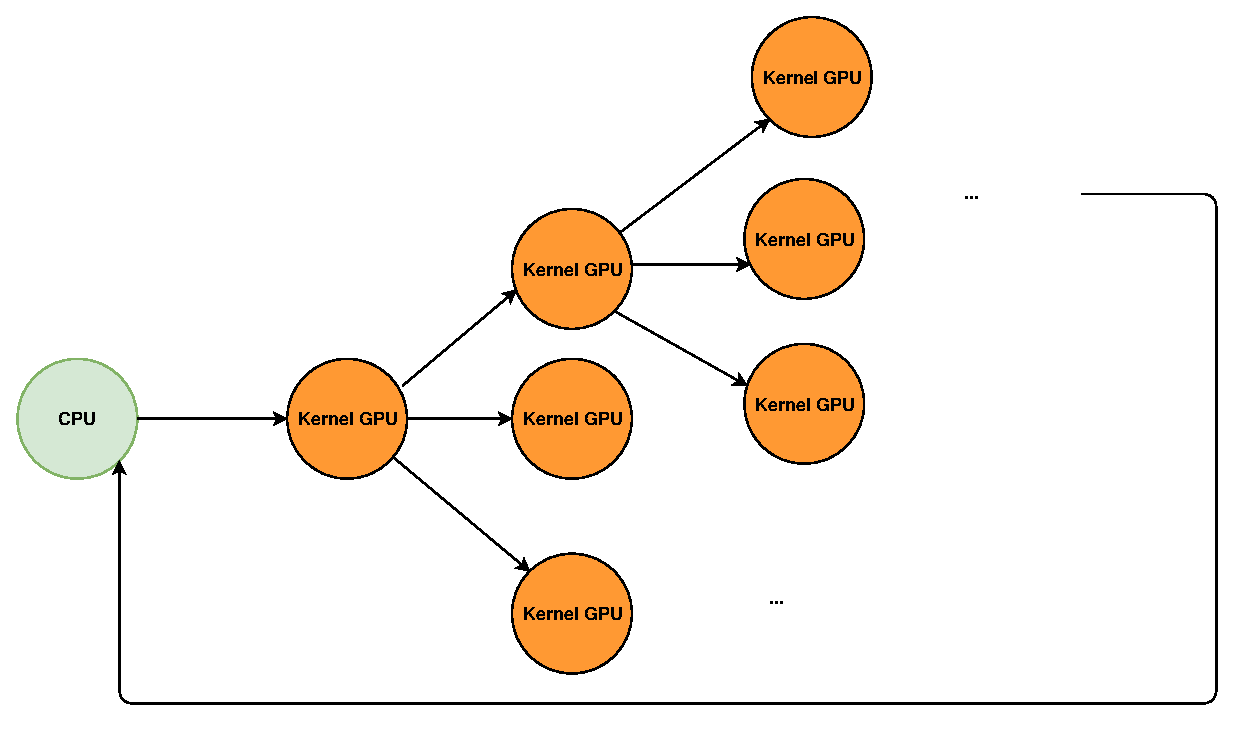
\includegraphics[scale=0.70]{figures/paralelismo_dinamico.eps}
 	\caption{Esquema conceptual del paradigma \textit{Dynamic Parallelism}}
 	\label{fig_Parelismodinamico}
 \end{figure}
 
 \subsection{Problemas de dominio tetra\'edrico}
 \label{sub_sec_ModTriple}
 
  En m\'ultiples \'areas cient\'ificas como la qu\'imica, f\'isica y biolog\'ia, existe un tipo de problema donde el dominio de datos en donde el computo se realiza puede ser, por un lado, el \'area bajo la linea diagonal interceptada por los ejes $x$ e $y$ formando un \'area triangular y que se puede modelar en superficies de dos dimensiones. Sin embargo, tambi\'en existe un problema donde su dominio puede formar un tetraedro de forma an\'aloga  al caso de 2D, el cual se puede modelar en superficies de 3D. Aqu\'i es donde nacen los problemas de dominio tetra\'edrico \cite{EffectTriplet1992} \cite{ThreadMapforSimplex2018}. Cada vez crece la necesidad de solucionar estos problemas de forma m\'as eficiente, dado a que al momento de mapear los datos existentes se genera una redundancia, esto se produce debido a que los datos que est\'an bajo de la diagonal, en el caso dos dimensiones, se repiten con los datos que est\'an por sobre la diagonal, haciendo que exista un c\'alculo innecesario ocupando m\'as recursos de los necesarios en la GPU. Esta redundancia de datos tambi\'en aparece  cuando se buscan todos los tr\'ios posibles de un conjunto de $n$ elementos, haciendo que en algunos de estos tr\'ios generen el mismo resultado, provocando la redundancia anteriormente mencionada. Un ejemplo de este tipo de problemas es el de las ecuaciones diferenciales parciales, cuyas funciones de frontera pueden formar una superficie de dominio tetra\'edrico y al hacer la simulaci\'on por diferencias finitas se genera la necesidad de descartar los c\'alculos que est\'an por sobre el plano diagonal. Por lo que resultar\'ia interesante encontrar una forma m\'as eficiente de trabajar con este tipo de problemas.
 





\section{Trabajo Relacionado}
\label{sec_trabajo_relacionado}

Los trabajos relacionados a este estudio tienen como eje central la b\'usqueda de formas  eficientes de trabajar con GPU en cuanto a tiempo de ejecuci\'on y espacio en memoria.

 C. A. Navarro y N. Hitschfeld, estudiaron \textit{td-problem (problema de dominio triangular)}\ en $\mathcal{R}^2$ \cite{GPUMaps2014}. Este trabajo se centra en hacer un an\'alisis comparativo de cuatro formas de mapeo de \textit{threads} de ejecuci\'on: \textit{bounding box (BB), upper-triangular mapping (UTM), rectangular box (RB) y recursive partition (REC)}. Adem\'as proponen un nuevo m\'etodo denominado $g(\lambda)$, este mapeo se basa en la propiedad de matriz triangulo inferior. Para este estudio se utilizaron tres m\'aquinas de Nvidia (GTX765M, GTX680, Tesla K40). De este estudio se lleg\'o a la conclusi\'on que este \'ultimo tiene un $17\%$ de mejora con respecto a \textit{bounding box (BB)}. Otro trabajo, presentado por Jin Hyuk Jung \cite{ExploStruct2007} mostr\'o como se puede explotar la rasterizaci\'on triangular de matrices sim\'etricas en GPU, resultando beneficioso en cuanto a rendimiento en comparaci\'on a algoritmos que son dise\~nados para CPU. 
	
 C. A. Navarro et al., plantearon y analizaron la posibilidad de realizar mapeos eficientes de forma recursiva (donde se podr\'ia aplicar \textit{dynamic parallelism}) en uno, dos, tres o $n$ dimensiones \cite{PossiRec2016}. En este trabajo se plante\'o un incremento de entre dos y seis veces de eficiencia utilizando algoritmos recursivos, sin embargo no se comprob\'o esta teor\'ia emp\'iricamente.

 Crist\'obal A. Navarro et al. \cite{ASurvey2014} explicaron los conceptos b\'asicos de la computaci\'on paralela y en especial en GPU. Explic\'o algunos ejemplos de aplicaci\'on que son ideales para sacarle provecho a la computaci\'on de alto rendimiento en GPU. Tambi\'en mencion\'o los problemas de mapeo de \textit{threads} en GPU dando a entender los conceptos con algunos ejemplos.

 Penporn Koanantakool et al., estudiaron los problemas en donde interact\'uan 3 cuerpos \cite{3body2014} y la necesidad para las ciencias como la f\'isica, qu\'imica o de los materiales para realizar algoritmos eficientes para realizar c\'alculos de gran escala que se produce gracias a cierta redundancia de datos (considerando que para el caso de dos dimensiones $f(i,j)=-f(j,i)$).




% E. Elsen et al. \cite{NBodySimulation2011} describieron lo ideales que son los problemas \textit{N-Body} para la arquitectura de la GPU, as\'i como tambi\'en la necesidad de que los algoritmos que trabajan con estos problemas sean eficientes, dado el alto grado de computo que implican estos problemas, tambi\'en para un uso optimo de los recursos de la GPU y realizar los c\'alculos en un menor tiempo. Otro trabajo propuesto por J. Bdorf et al. \cite{ASparceGrav2011}, tambi\'en propuso un nuevo algoritmo de \'arbol NBody gravitatorio para GPU. Este algoritmo present\'o una mejora de rendimiento  de 20x con respecto a c\'odigo creado para CPU.
% Q. Avril et al. \cite{FastCollision2012} propusieron un algoritmo que busca utilizar los recursos de la GPU de forma eficiente, capaz de explotar al m\'aximo el paralelismo y los sub-procesos m\'ultiples para resolver problemas de pares de objetos no colisionantes en simulaciones din\'amicas a gran escala.

 D. Man et al. \cite{AGPUEuclideanDis} propusieron mejorar la eficiencia de la GPU desde el punto del vista de la velocidad de acceso a memoria, proponiendo un algoritmo basado en el mapa de distancias euclidiano donde logran una mejora de aceleraci\'on en un factor de 52 veces por sobre la implementaci\'on de un algoritmo secuencial. Otro trabajo mostrado por Z. Ying et al. \cite{DNAGPU2011} busc\'o acelerar el programa DNADIST utilizando openCL, con el fin de explotar la gran capacidad de computo de una GPU. En este trabajo se logr\'o una aceleraci\'on de 12 veces.

 

Es importante mencionar que cada uno de estos trabajos manifiestan un inter\'es por encontrar formas eficientes de trabajar en GPU, tanto en tiempo y espacio. A pesar de las mejoras que se consiguen en rendimiento en cuanto a c\'alculos de gran escala, nuestra hip\'otesis es que a\'un es posible seguir mejorando ya sea optimizando ciertos algoritmos o encontrando nuevas formas de explotar los n\'ucleos de la GPU. 

\section{Soluci\'on propuesta}
\label{sec_implementacion}


Esta secci\'on se enfoca en explicar el desarrollo de un algoritmo usando el paradigma de \textit{dynamic parallelism} el cual de ahora en adelante se llamar\'a \textit{m\'etodo DP}. Para el desarrollo de este algoritmo se utiliz\'o NVidia CUDA \cite{Nvidia2016}.

A continuaci\'on se explica el m\'etodo DP, con el estudio de sus respectivos par\'ametros. 


\subsection{M\'etodo DP}



El algoritmo propuesto (ver \ref{ssec_Metodo_PD}) se basa en la alternativa de mapeo \textit{3-simplices} \cite{PossiRec2016}, considerando la dimensi\'on del problema o cubo de tama\~no de arista $n$. Se aplic\'o \textit{dynamic parallelism} es para formar un tetraedro constituido por cubos, el primer \textit{kernel} de recursi\'on forma un cubo de tama\~no $n/2$ (cubo de color rojo en Figura \ref{fig_diagram_dp}), del cual se desprenden tres \textit{streams}\footnote{En CUDA las ramas de recursi\'on se asocian a un \textit{stream} distinto, esto permite lanzar varios kernel de recursi\'on paralelamente, a trav\'es de \textit{pipeline} de forma concurrente en la GPU.}, un \textit{stream} hacia el eje \textit{x}, otro hacia el eje \textit{y} y el \'ultimo hacia el eje \textit{z}. De cada una de estas ramas recursivamente se formar\'an  cubos de la mitad de su tama\~no anterior, hasta completar en la condici\'on $x+y>z$.

Dado a las caracter\'isticas de la geometr\'ia de los datos y el modelo de computo que posee la GPU, se debieron elegir ciertos par\'ametros para el correcto funcionamiento del algoritmo. Debido a un problema de la geometr\'ia de un tetraedro, hay cubos que sobresalen del plano diagonal. Para contrarestar esto, se llenan los espacios vac\'ios que quedan en la diagonal lanzando un \'ultimo \textit{kernel} dedicado a llenar estos espacios y a eliminar los \textit{threads} sobrantes por el plano diagonal. 
\begin{figure}[H]
	\centering
	\includegraphics[trim = 10mm 80mm 20mm 5mm, clip,scale=0.75]{figures/Diagrama_PD.eps}
	\caption{Representaci\'on gr\'afica de m\'etodos DP}
	\label{fig_diagram_dp}
\end{figure}
Tomando como referencia la Figura \ref{fig_diagram_dp} y considerando un problema de tama\~no $n$, se puede modelar una ecuaci\'on que representa la recursividad de este m\'etodo. Sea $V(D_{n})$ el volumen del dominio de tama\~no $n$ o tetraedro y $V(C_{n})$ el volumen del cubo de tama\~no $n$, entonces se puede considerar que el volumen del tetraedro se puede modelar en la ecuaci\'on \ref{ecuacion_Volumen}.



\begin{equation}
\label{ecuacion_Volumen}
V(D_{n}) =  V(C_{n/2}) + 3V(D_{n/2})
\end{equation}
\begin{equation}
\label{ecuacion_Vol_corte}
\textbf{}V(D_{n_{c}})=V(C_{n_{c}})
\end{equation}
 
 
 
 Si se analiza la ecuaci\'on \ref{ecuacion_Volumen}, vemos que el primer termino corresponde al volumen del cubo inicial de tama\~no $n/2$ para luego sumar el volumen de tres de los cubos peque\~nos que se forman de tama\~no $(n/2)/2$ (como tambi\'en se puede ver en Figura \ref{fig_diagram_dp}) con condici\'on de corte en la ecuaci\'on \ref{ecuacion_Vol_corte}, donde $n_{c}$ corresponde a un $n$ de corte ideal, para no continuar ejecutando recursiones. La elecci\'on de este par\'ametro, se explica a continuaci\'on.
 

 
\subsection{Elecci\'on de $n_{c}$ }
\label{Exp_nCORTE}


En teor\'ia, el n\'umero de recursiones es $log_{2} n$, sin embargo, a partir de cierto valor $n<n_{c}$ los sub-problemas son muy peque\~nos y no alcanzan a generar suficiente trabajo para la GPU. Para ello debe existir una condici\'on para detener la ejecuci\'on de las recursiones. En teor\'ia la ejecuci\'on de las recursiones deber\'ia detenerse cuando el tama\~no del cubo sea igual o menor a uno. Al detener la recursi\'on tempranamente, quedan espacios en el tetraedro que a\'un no fueron accedidos por alg\'un \textit{thread}. Este fen\'omeno se convierte en un problema que debe ser solucionado. La soluci\'on propuesta consiste en que al finalizar la \'ultima recursi\'on se generen cubos de igual tama\~no a los de la \'ultima recursi\'on y se ubiquen a los lados de los cubos de la \'ultima recursi\'on. Se debe encontrar un $n$ de corte ideal (denominado de ahora en adelante $n_{c}$ como se ve en ecuaci\'on \ref{ecuacion_Vol_corte}) que alcance a cubrir la totalidad del problema y que afecte en lo m\'as m\'inimo el rendimiento de la GPU. Es decir, una vez que la recursi\'on llega a $n=n_{c}$ se invoca otro \textit{kernel} que se encargue de cubrir la diagonal. Esto sucede en paralelo en todas la ramas de la recursi\'on.



 Para la elecci\'on de $n_{c}$ se consider\'o hacer pruebas en dos m\'aquinas (ver tablas \ref{table_gtx1050_nc} y \ref{table_TeslaK40_nc}), obteniendo los resultados en la Figura \ref{fig_N_Corte_Ideal}. En este gr\'afico se puede notar que el eje $x$ corresponde tama\~no de problema $n$. Para cada $n$, se midi\'o el tiempo dado el par\'ametro de $n_{c}$ considerando el tiempo por cada tama\~no de problema.
 
  \begin{figure}[H]
  	\centering
  	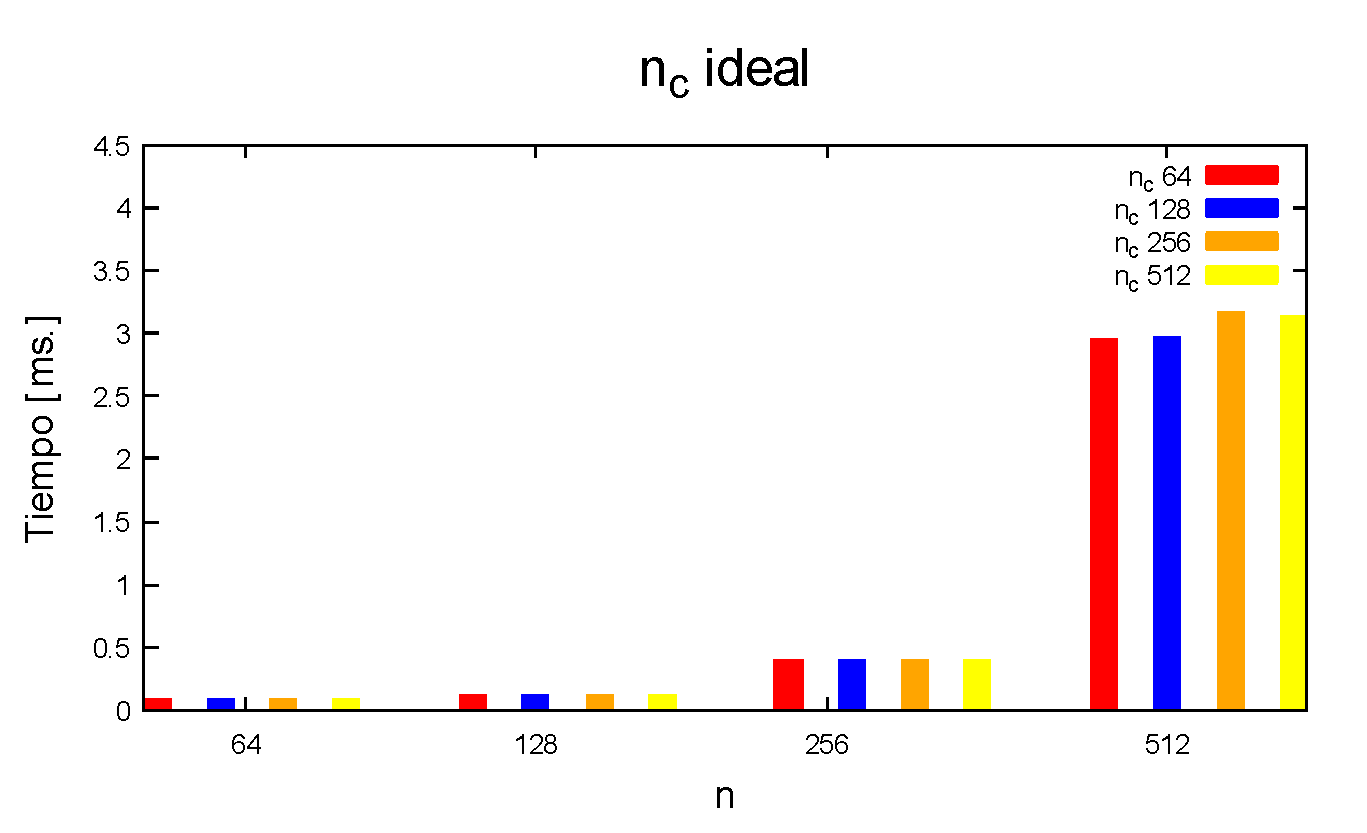
\includegraphics[scale=0.45]{figures/nideal_aphopis.eps}
  	\caption{Tiempo de ejecuci\'on  para distintas combinaciones de $n$ y $n_{c}$. La mayor reducci\'on de tiempo se obtiene en $n_{c}=128$ para todo $n$. }
  	\label{fig_N_Corte_Ideal}
  \end{figure}
  
 \begin{table}[H]
 	\normalsize
 	\caption{M\'aquina de prueba uno para determinar $n_{c}$.}
 	\begin{center}
 		\begin{tabular}{|c|r|}
 			\hline
 			Dispositivo	&	Modelo\\
 			\hline
 			GPU	&	GTX 1050 Ti Pascal, GP107, 640 cores, 2GB\\
 			CPU	&	AMD FX-8350 8-core\\
 			RAM	&	8GB RAM\\
 			\hline
 		\end{tabular}
 	\end{center}
 	\label{table_gtx1050_nc}
 \end{table}
 
 \begin{table}[H]
 	\normalsize
 	\caption{M\'aquina de prueba dos para determinar $n_{c}$.}
 	\begin{center}
 		\begin{tabular}{|c|r|}
 			\hline
 			Dispositivo	&	Modelo\\
 			\hline
 			GPU	&	NVIDIA Tesla K40c,2880 cores, 12 GB\\
 			CPU	&	Procesador Intel® Xeon® E5-2640\\
 			RAM	&	128 GB\\
 			\hline
 		\end{tabular}
 	\end{center}
 	\label{table_TeslaK40_nc}
 \end{table}
 
 Con los resultados arrojados por el gr\'afico, se decidi\'o tomar en consideraci\'on las \'ultimas potencias de dos (64, 128, 256 y 512) que son las m\'as altas y donde m\'as se perciben los espacios en blanco. Se seleccion\'o 128 como $n_{c}$, a pesar de que 64 tiene valores similares con un margen muy estrecho  de diferencia con 128, se eligi\'o por ser un $n$ alto que asegura el llenado de los espacios en blanco y que no afecta con creces el rendimiento del m\'etodo.
 




\subsection{Elecci\'on de \textit{BlockSize} ideal}
\label{ele_blocksize}

Como se mencion\'o anteriormente en la secci\'on \ref{sub_sec_ModCuda}, en CUDA, los \textit{threads} de ejecuci\'on se organizan en una jerarquizaci\'on espacial, donde la unidad b\'asica es el \textit{thread}. Estos \textit{threads} se organizan en \textit{blocks} de tama\~no $BlockSize \times BlockSize \times BlockSize$. Los \textit{blocks} se organizan en un \textit{Grid} o grilla.

El tama\~no de \textit{block} ideal es aquel que maximiza grado de paralelismo por \textit{kernel} ejecutado, para esto se debe entender que CUDA organiza los \textit{threads} como se describi\'o anteriormente (ver Figura \ref{fig_Jerarquia}).
Para la elecci\'on del \textit{BlockSize} ideal se tom\'o en consideraci\'on el $n_{c}$ cuyo resultado fue 128. Se hicieron mediciones donde se tomaron los \textit{BlockSize} de tama\~no dos, cuatro y ocho \textit{threads}, que son los tama\~nos admitidos por CUDA. 



Las mediciones realizadas dieron como resultado un \textit{BlockSize} ideal de ocho \textit{threads} como se puede ver en el gr\'afico de la Figura \ref{fig_Block_size_i}. Esto es comprensible, dado a la arquitectura de una GPU mientras m\'as \textit{threads} se ejecutan por \textit{block}, m\'as \textit{threads} se paralelizan, ya que los \textit{streaming multiprocessor} de la GPU ejecutan un \textit{block} en un instante dado y para que sea saturado estos deben ser del orden de 256, 512 o 1024 \textit{threads} por \textit{block}. Este comportamiento en el tama\~no de \textit{BlockSize} aplica para todos los casos ya que se comprob\'o que en las cuatro m\'aquinas donde se realiz\'o este estudio (ver tablas \ref{table_titanx}, \ref{table_gtx1050}, \ref{table_TeslaK40}, \ref{table_TeslaV100}), el ideal es un \textit{BlockSize} de ocho. Esto implica que cada \textit{block} ejecut\'andose en GPU, ejecuta $8 \times 8 \times 8=512 $ \textit{threads} de forma paralela.

\begin{figure}[H]
	\centering
	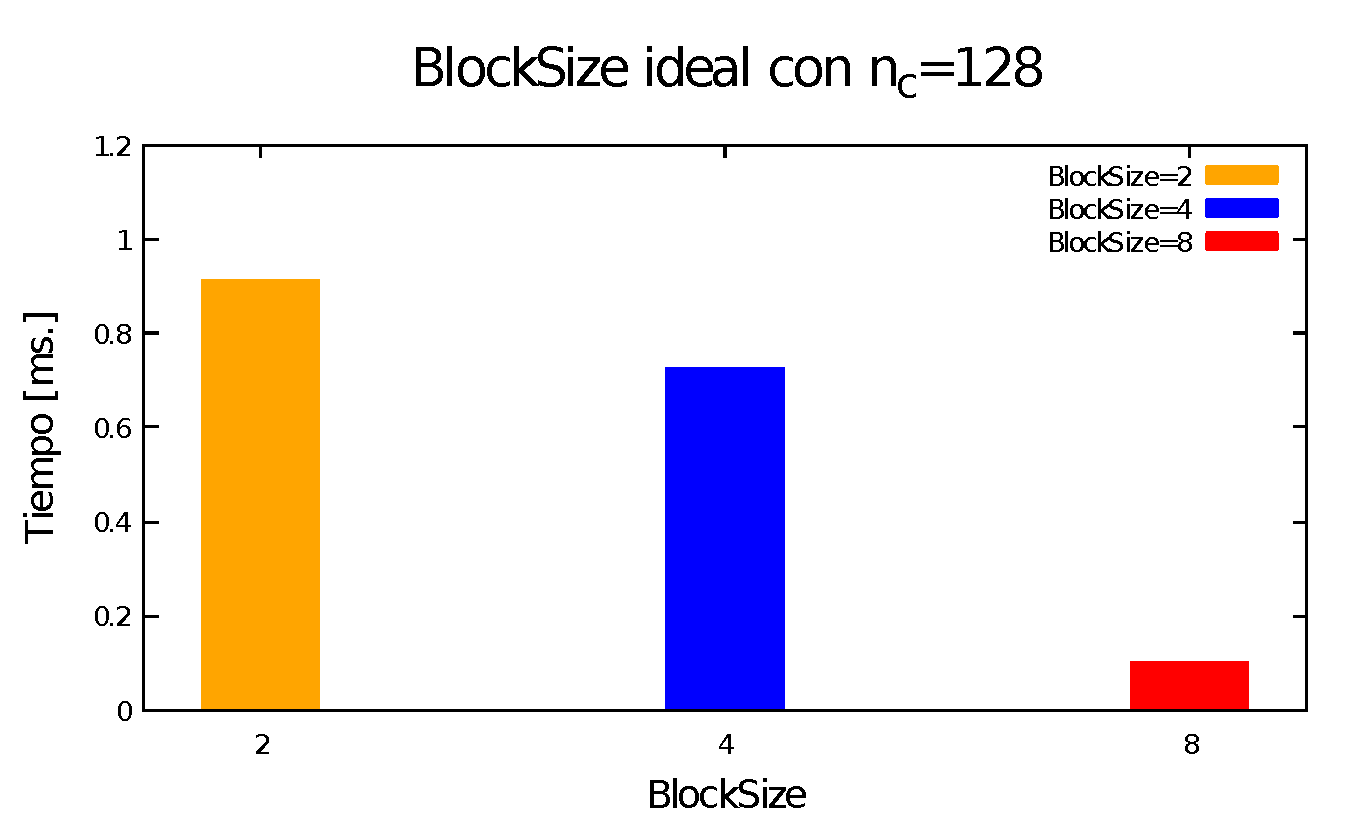
\includegraphics[scale=0.45]{figures/BSideal.eps}
	\caption{Tiempo de ejecuci\'on en funci\'on del \textit{BlockSize}, el valor ideal es ocho.}
	\label{fig_Block_size_i}
\end{figure}

\subsection{Implementaci\'on}

En esta subsecci\'on se explica la implementaci\'on del algoritmo que se encuentra en la secci\'on Anexos \ref{ssec_Metodo_PD} correspondiente al m\'etodo DP.

El \textit{kernel} que se program\'o en CUDA recibe como par\'ametro de entrada una matriz de tama\~no $n\times n \times n$, la coordenada de inicio del primer cubo en $\mathcal{R}^3$, el lado $n$ del tetraedro, $n_{c}$ y el \textit{BlockSize}. Los \textit{threads} son mapeados a una regi\'on c\'ubica dentro del tetraedro. En este punto se crean dos identificadores de \textit{threads}, uno para saber la coordenada absoluta en los datos y la segunda para saber el identificador del thread relativo a su \textit{kernel}. En este momento se puede escribir el primer cubo de tama\~no de arista $n/2$ mapeado al dominio de datos. Luego pueden pasar dos situaciones prueba: (1) se termina la recursi\'on porque el tama\~no del sub-problema es muy peque\~no y se procede a llenar la diagonal  pendiente con un \'ultimo \textit{kernel} especial que no es recursivo o (2) se crean tres ramas de recursi\'on (usando \textit{streams} distintos) y para ejecutar sub-problemas de $n/2\times n/2 \times n/2$. Se defini\'o que cada \textit{stream} sea \textit{Non-Blocking} ya que esto permite generar concurrencia en los kernels a ejecutar. Cabe destacar que los \textit{streams} son llamados por un solo \textit{thread} del \textit{kernel} el que tiene identificador 0, ya que de lo contrario generar\'ian una cantidad enorme e innecesaria de \textit{kernels} recursivos. 






\section{Resultados de rendimiento}
\label{sec_resultado}
En esta secci\'on se describen los resultados obtenidos en las distintas pruebas de rendimiento realizadas. Para obtener los resultados se consideraron cuatro m\'aquinas (ver tablas \ref{table_titanx}, \ref{table_gtx1050}, \ref{table_TeslaK40}, \ref{table_TeslaV100}), con distintas GPUs y arquitecturas de estas mismas. Para estudiar el m\'etodo propuesto en este trabajo, se compara con el m\'etodo fuerza bruta (\textit{ver \ref{ssec_fuerza_bruta}}) basado en \textit{bounding box} \cite{PossiRec2016}, el cual consiste en mapear los \textit{threads} de GPU de forma directa. Es decir, se recorre cada uno de los puntos del cubo, descartando aquellos que cumplen con la condici\'on de \textit{($x+y > z$)}. No se consider\'o el tiempo de traspaso de datos entre \textit{device} y \textit{hosts}, ya que pasa a ser despreciable cuando la GPU reutiliza varias veces los datos alojados en la memoria de GPU. Es decir, que el traspaso entre \textit{host} y \textit{device} sucede una sola vez, mientras que el c\'alculo o computo en los n\'ucleos de la GPU sucede muchas veces.



 \begin{table}[H]
	\normalsize
	\caption{Especificaciones de hardware de la m\'aquina 1.}
	\begin{center}
		\begin{tabular}{|c|r|}
			\hline
			Dispositivo	&	Modelo\\
			\hline
			GPU	&	Titan-X Pascal, GP102, 3584 cores, 12GB\\
			CPU	&	Intel i7-6950X 10-core Broadwell\\
			RAM	&	128GB DDR4 2400MHz\\
			\hline
		\end{tabular}
	\end{center}
	\label{table_titanx}
\end{table}

\begin{table}[H]
	\normalsize
	\caption{Especificaciones de hardware de la m\'aquina 2.}
	\begin{center}
		\begin{tabular}{|c|r|}
			\hline
			Dispositivo	&	Modelo\\
			\hline
			GPU	&	GTX 1050 Ti Pascal, GP107, 640 cores, 2GB\\
			CPU	&	AMD FX-8350 8-core\\
			RAM	&	8GB RAM\\
			\hline
		\end{tabular}
	\end{center}
	\label{table_gtx1050}
\end{table}

\begin{table}[H]
	\normalsize
	\caption{Especificaciones de hardware de la m\'aquina 3.}
	\begin{center}
		\begin{tabular}{|c|r|}
			\hline
			Dispositivo	&	Modelo\\
			\hline
			GPU	&	NVIDIA Tesla K40c,2880 cores, 12 GB\\
			CPU	&	Procesador Intel® Xeon® E5-2640\\
			RAM	&	128 GB\\
			\hline
		\end{tabular}
	\end{center}
	\label{table_TeslaK40}
\end{table}

\begin{table}[H]
	\normalsize
	\caption{Especificaciones de hardware de la m\'aquina 4.}
	\begin{center}
		\begin{tabular}{|c|r|}
			\hline
			Dispositivo	&	Modelo\\
			\hline
			GPU	&	Tesla V100-SXM2, 5120 cores, 16 GB \\
			CPU	&	Intel(R) Xeon(R) CPU E5-2686 v4 @ 2.30GHz\\
			RAM	&	128GB \\
			\hline
		\end{tabular}
	\end{center}
	\label{table_TeslaV100}
\end{table}
 Se utilizan los par\'ametros anteriormente encontrados en cada una de las m\'aquinas por igual. Cada \textit{kernel} de la recursi\'on escribe un valor constante en su regi\'on correspondiente en el tetraedro. Cuando todos los \textit{kernels} recursivos terminan, el resultado es un tetraedro escrito completamente. Para el caso de la fuerza bruta se escribe la misma constante utilizando el \textit{bounding box}. Independientemente del m\'etodo escogido el tiempo de ejecuci\'on de una instancia se obtiene promediando 180 ejecuciones de kernel. Como m\'etrica final se saca el tiempo promedio de  10 instancias lo que equivale a un promedio de promedios. Este proceso de medici\'on entrega tiempos estables y con bajo error est\'andar. Este \textit{benchmark}  se realiza por cada $n$. El proceso se iter\'o haciendo variar el tama\~no de \textit{n} del problema comenzando desde $n=8$ y terminando en $n=512$ con intervalos de 8 unidades.
 
 Como m\'etrica de rendimiento se utiliza el tiempo de ejecuci\'on arrojado en cada una de las iteraciones para posteriormente graficar la aceleraci\'on ($A_{DP}$) \cite{ASurvey2014}, cuyo valor se define como: 
 \begin{equation}
 \label{ecuacion_Speed_Up}
 \textbf{}A_{PD}=\dfrac{T_{FB}}{T_{DP}},
 \end{equation}
 Que corresponde a la raz\'on entre el tiempo obtenido del \textit{M\'etodo DP} ($T_{DP}$) y el m\'etodo \textit{Fuerza bruta} ($T_{FB}$).\\
 En la Figura \ref{fig_Nvidiagtx}, donde se utiliza la m\'aquina descrita en la Tabla \ref{table_gtx1050}, se observa que el m\'etodo \textit{fuerza bruta}, considerando que es una m\'aquina de gama media, es mejor que el m\'etodo DP logrando una aceleraci\'on aproximada de  entre 0.7 y 0.8. Volvi\'endose relativamente constante a partir de $n=128$. En la Figura \ref{fig_Ace_Pascal}, donde se utiliza la m\'aquina descrita en \ref{table_titanx}, se puede observar una situaci\'on similar a la mencionada anteriormente. La aceleraci\'on comienza a permanecer constante en $n=220$ aproximadamente y los valores de este oscilan entre 0.6 y 0.7. En la Figura \ref{fig_Ace_teslaK40}, donde se utiliza la m\'aquina descrita en la Tabla \ref{table_TeslaK40}, no se presenta una situaci\'on muy lejana a las anteriormente mencionadas, los valores de la aceleraci\'on comienzan a volverse constantes a partir de $n=140$ aproximadamente y sus valores oscilan entre 0.7 y 0.9.
 

 

 
 En la Figura \ref{fig_Ace_Volta}, donde se utiliza la m\'aquina descrita en la Tabla \ref{table_TeslaV100}, es donde se presenta la mayor diferencia y variaciones de aceleraci\'on frente a las otras m\'aquinas estudiadas. A partir de $n=128$ se observa un notorio incremento en la aceleraci\'on. Hasta $n>256$ este valor oscila entre $1\times$ y $2\times$, sin embargo a partir de 256 este tiene una abrupta crecida oscilando entre $2.4\times$ y $3.1\times$ aproximadamente.
 

 
 Los resultados de rendimiento arrojados por cada m\'aquina permiten conocer y analizar el comportamiento del m\'etodo PD frente a fuerza bruta. Por otro lado, es posible inferir que existe una influencia importante de la arquitectura de la GPU en el comportamiento del m\'etodo.
 \begin{figure}[H]
 	\centering
 	\begin{subfigure}[b]{0.475\textwidth}
 		\centering
 		\includegraphics[width=\textwidth]{figures/ace_Nvidia_gtx.eps}
 		\caption{Gr\'afico de aceleraci\'on en NVidia GeForce GTX 1050 Ti}
 		
 		\label{fig_Nvidiagtx}
 	\end{subfigure}
 	\hfill
 	\begin{subfigure}[b]{0.475\textwidth}
 		\centering 
 		\includegraphics[width=\textwidth]{figures/Ace_pascal.eps}
 		\caption{Gr\'afico de aceleraci\'on en Titan X(Pascal)}
 	   
 		\label{fig_Ace_Pascal}
 	\end{subfigure}
 	\vskip\baselineskip
 	\begin{subfigure}[b]{0.475\textwidth} 
 		\centering 
 		\includegraphics[width=\textwidth]{figures/ace_teslak40.eps}
 		\caption{Gr\'afico de aceleraci\'on en Tesla K40c}
 	    
 		\label{fig_Ace_teslaK40}
 	\end{subfigure}
 		\quad
 		\begin{subfigure}[b]{0.475\textwidth}   
 			\centering 
 			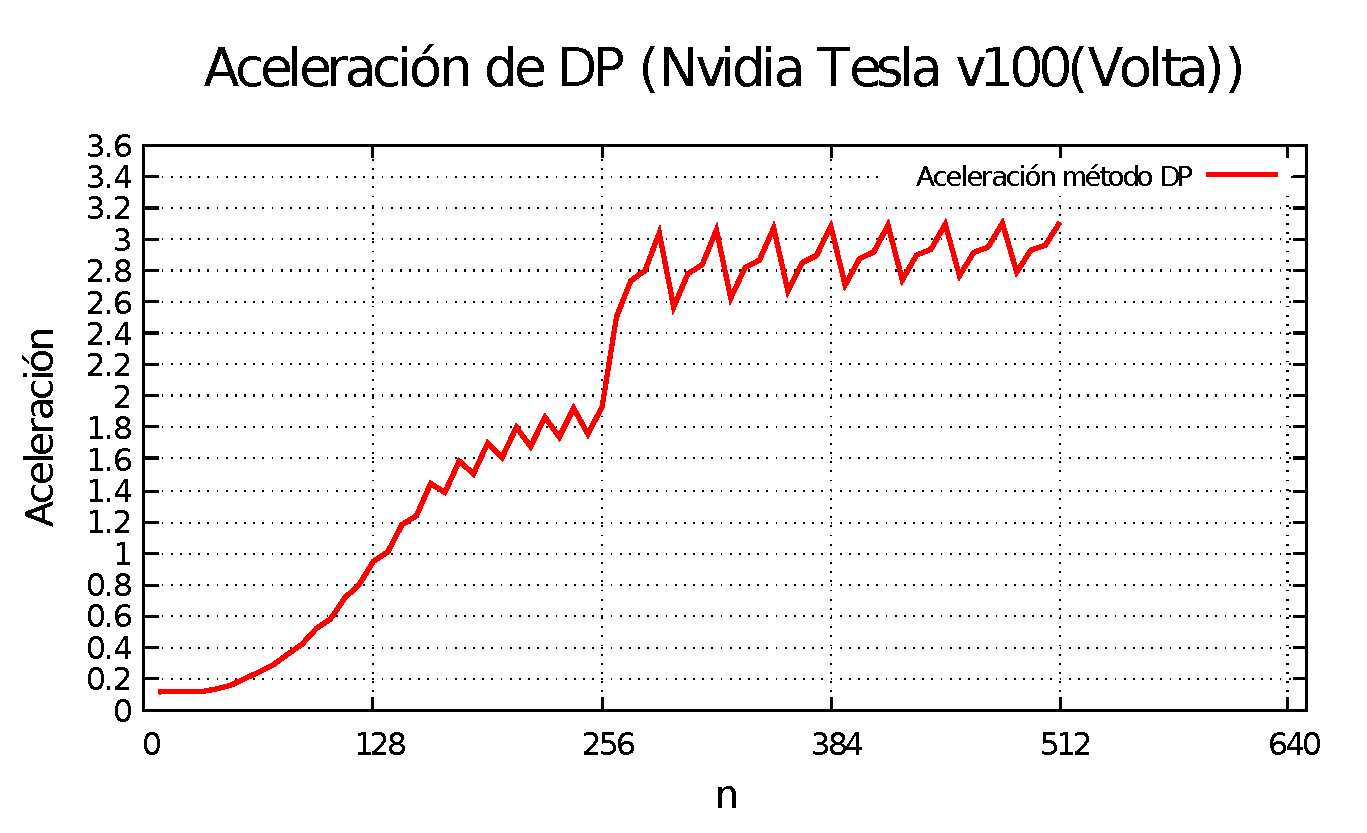
\includegraphics[scale=0.4]{figures/ace_Volta.eps}
 			\caption{Gr\'afico de aceleraci\'on en Tesla V100(Volta)}
 			   
 			\label{fig_Ace_Volta}
 			
 	\end{subfigure}
 	
 	\caption[ Gr\'aficos de aceleraci\'on de las  cuatro m\'aquinas estudiadas. ]
 	{\small Gr\'aficos de aceleraci\'on de las  cuatro m\'aquinas estudiadas.} 
 	\label{Graf_aceleracion}
 \end{figure}

 




\section{Discusi\'on}
\label{sec_discusion}

 
De la secci\'on anterior (\ref{sec_resultado}) se pudo observar que en tres de las m\'aquinas estudiadas no hay grandes diferencias de comportamiento entre GPUs con respecto a la utilizaci\'on de \textit{dynamic parallelism}, sigue sobresaliendo el m\'etodo de mapeo de \textit{threads} fuerza bruta. Esto se debe a que quiz\'as hay una menor cantidad de c\'alculos que cada \textit{thread} mapeado debe hacer con respecto a la cantidad de \textit{threads} que se deben descartar. Donde se pudo notar un comportamiento similar pero con mayor variaci\'on de tiempo, fue en la GPU Titan X con arquitectura Pascal, donde el valor de la aceleraci\'on oscil\'o entre $0.6\times$ y $0.7\times$. Cabe destacar que esta oscilaci\'on se podr\'ia deber a que hay valores de $n$ donde se deben ajustar los c\'alculos dado a una inexactitud en la divisi\'on que no coincid\'ian con el algoritmo planteado. Es decir, dentro del algoritmo hay divisiones que no son exactas por el hecho de que su resultado es un n\'umero impar o no entero, para ello se hicieron c\'alculos de redondeos para ciertos $n$ que presentan ese problema. Esto, en alguna medida debi\'o afectar el rendimiento del algoritmo, por lo tanto quiz\'as sea posible optimizar el c\'odigo para encontrar una soluci\'on que minimice este c\'alculo.
  
 El principal hallazgo, es la mejora de rendimiento y eficiencia utilizando \textit{dynamic parallelism} en la m\'aquina con GPU Tesla V100. Mejora que puede ser hasta  $\sim 3\times$. Se puede inferir que este crecimiento puede deberse a que dentro de las cuatro GPUs seleccionadas para este estudio, es la m\'as reciente y su arquitectura est\'a hecha para potenciar la computaci\'on de alto rendimiento. Algo que se puede observar en este gr\'afico, es que se produce un abrupto crecimiento en $n=256$ aproximadamente. Hay muchos factores que podr\'ian desencadenar este comportamiento, por ejemplo, podr\'ia ser atribuible a una elecci\'on de par\'ametros m\'as exactos para cada m\'aquina seleccionada, por ejemplo, quiz\'as para esta m\'aquina el valor de $n_{c}$ deber\'ia ser 256 y no 128. Este comportamiento merece ser estudiado m\'as a fondo a futuro.
 
 Otro comportamiento observado en este estudio, es la diferencia que existe al ejecutar el m\'etodo fuerza bruta en la m\'aquina con GPU tesla V100 (Volta), en comparaci\'on con el resto de las m\'aquinas analizadas. Como se puede observar en la Figura \ref{fig_compa_volta} donde se comparan los tiempos de ejecuci\'on, el m\'etodo fuerza bruta gana con respecto al m\'etodo DP, donde el tiempo de ejecuci\'on para $n=512$ no alcanza a ser m\'as 0.6 ms. En contraste con la GPU Tesla V100, como podemos ver en la Figura \ref{fig_Carbon_compa} pierde con creces, de hasta casi $10\times$. Ocurre una situaci\'on muy similar si comparamos el gr\'afico de la GPU Tesla V100 con las otras GPUs analizadas, por lo que resultar\'ia interesante descubrir por qu\'e ocurri\'o esto solo en esta GPU y no en las otras estudiadas.



\begin{figure}[H]
	\centering
	\begin{subfigure}[b]{0.475\textwidth}
		\centering
		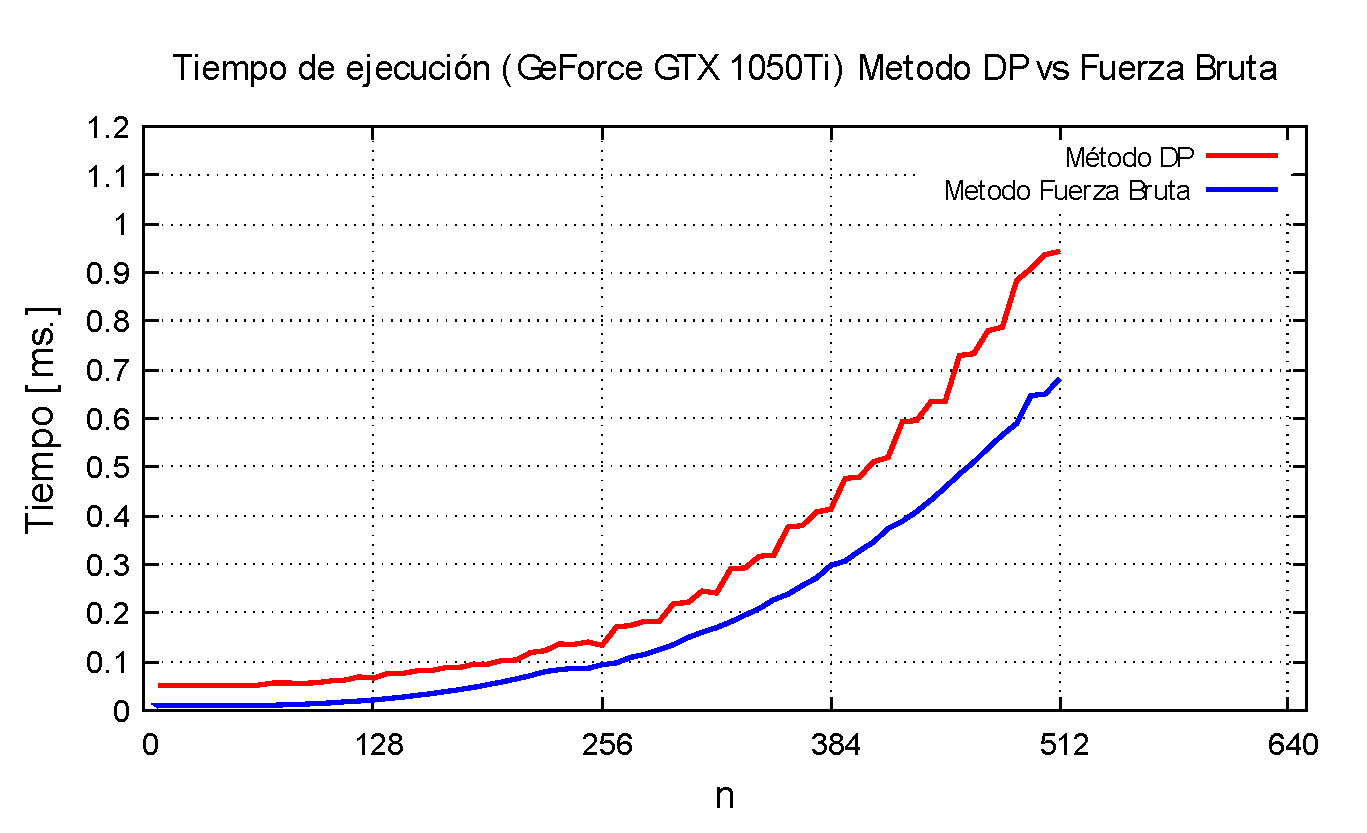
\includegraphics[width=\textwidth]{figures/carbon_compa.eps}
		\caption{Gr\'afico de tiempo vs. $n$ en NVidia GeForce GTX 1050 Ti}
		\label{fig_compa_volta}
	\end{subfigure}
	\hfill
	\begin{subfigure}[b]{0.475\textwidth}
		\centering 
		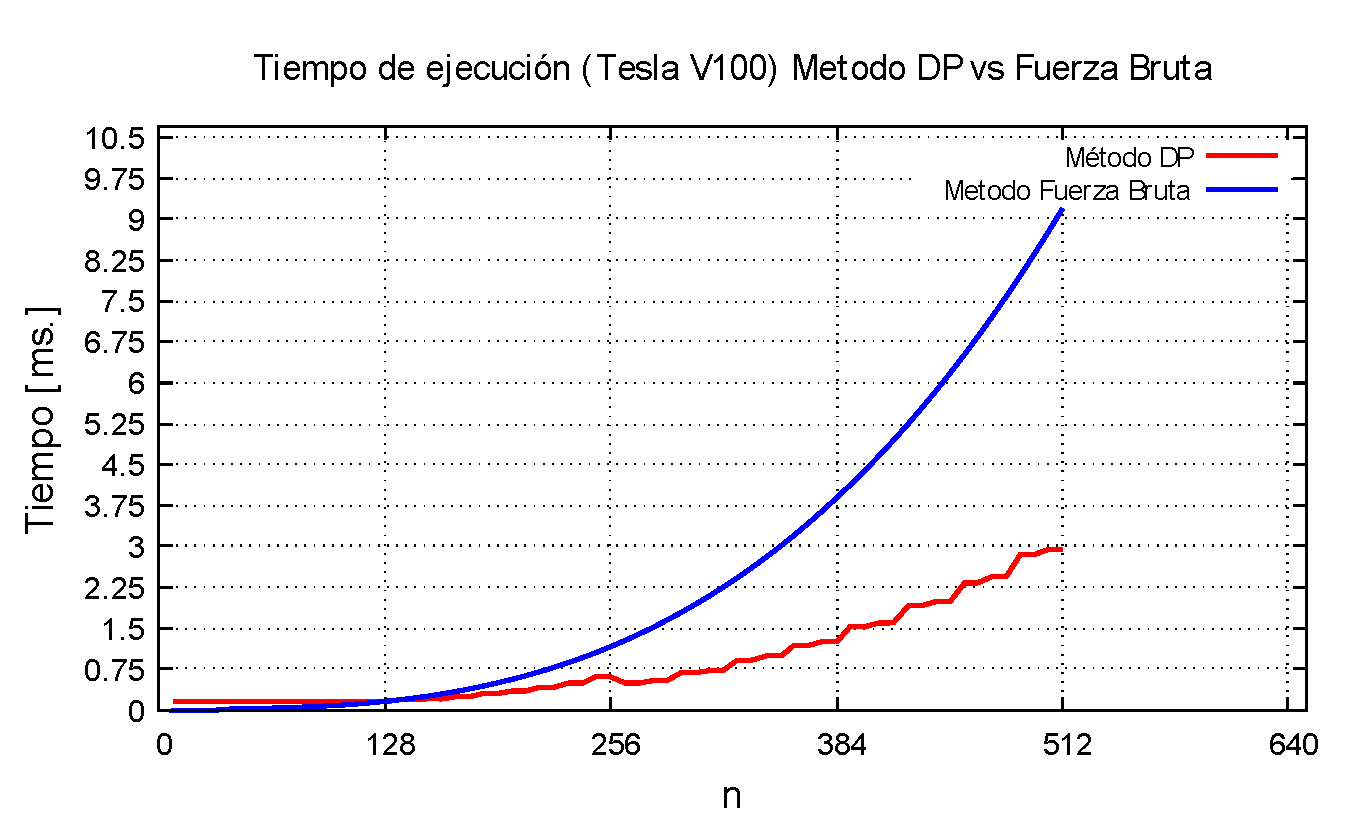
\includegraphics[width=\textwidth]{figures/Volta_comp.eps}
		\caption{Gr\'afico de tiempo vs. $n$ en Tesla V100}
		\label{fig_Carbon_compa}
	\end{subfigure}
 	\caption[ Gr\'aficos de comparaci\'on entre m\'aquina Tesla V100 con GTX 1050Ti. ]
{\small Gr\'aficos de comparaci\'on entre m\'aquina Tesla V100 con GTX 1050Ti.} 
\label{Graf_compa}
\end{figure}




\section{Conclusi\'on}
Retomando la pregunta de investigaci\'on planteada en la introducci\'on de este articulo ?`Pueden las \'ultimas tecnolog\'ias de GPU, tales como \textit{Dynamic Parallelism}, reducir la cantidad de \textit{threads} para dominios de tetraedro en tres dimensiones y entregar una mejora en rendimiento como consecuencia? Respondiendo a esta pregunta, en este estudio, solo se lograron resultados positivos en una GPU con arquitectura Volta (Tesla V100), logrando una mejora de $\sim 3\times$, por lo que ser\'ia interesante descubrir por qu\'e raz\'on solo se logr\'o una mejora en esta GPU. Adem\'as, del comportamiento curioso que tuvo esta arquitectura con el m\'etodo fuerza bruta fue mucho m\'as lento que en otras m\'aquinas. Considerando los resultados se puede deducir que el funcionamiento de \textit{dynamic parallelism} var\'ia de acuerdo a la arquitectura de la GPU. Sin embargo tambi\'en puede que esto sea debido a la variaci\'on de par\'ametros utilizados como $n_{c}$ o \textit{BlockSize}. Los resultados de este estudio no est\'an muy lejos a los que propone y estima C. A. Navarro et al. \cite{PossiRec2016}, quien afirma que se podr\'ia lograr una posible mejora de rendimiento variando entre $2\times$ y $6\times$.
 

En este estudio se utilizaron valores iguales para cada equipo asumiendo un comportamiento similar en todas las m\'aquinas donde se realiz\'o este estudio. Por lo que cabe la posibilidad de que para cada arquitectura y GPU se deba realizar un estudio previo para determinar la existencia de los valores ideales de \textit{BlockSize} y de $n_{c}$ espec\'ificos. Si esto es as\'i, podr\'ian existir cambios en el rendimiento en lo que se refiere a tiempo de ejecuci\'on del algoritmo para la resoluci\'on de un problema de dominio tetra\'edrico.

 Se demostr\'o emp\'iricamente que \textit{dynamic parallelism} es una t\'ecnica que no puede ser descartada totalmente, se puede aprovechar bastante si se encuentra la arquitectura adecuada para su uso. Se pudo notar la gran ventaja que tiene esta t\'ecnica en arquitectura Volta de NVidia. La arquitectura Volta es una de las m\'as recientes que desarroll\'o Nvidia, lo que demuestra que si en esta m\'aquina se encontr\'o que es conveniente utilizar \textit{dynamic parallelism}, a\'un queda mucho por descubrir y mejorar en esta tecnolog\'ia. 







% trigger a \newpage just before the given reference
% number - used to balance the columns on the last page
% adjust value as needed - may need to be readjusted if
% the document is modified later
%\IEEEtriggeratref{8}
% The "triggered" command can be changed if desired:
%\IEEEtriggercmd{\enlargethispage{-5in}}

% references section

% can use a bibliography generated by BibTeX as a .bbl file
% BibTeX documentation can be easily obtained at:
% http://www.ctan.org/tex-archive/biblio/bibtex/contrib/doc/
% The IEEEtran BibTeX style support page is at:
% http://www.michaelshell.org/tex/ieeetran/bibtex/
%\bibliographystyle{IEEEtran}
% argument is your BibTeX string definitions and bibliography database(s)
%\bibliography{IEEEabrv,../bib/paper}
%
% <OR> manually copy in the resultant .bbl file
% set second argument of \begin to the number of references
% (used to reserve space for the reference number labels box)
%\bibliographystyle{plain}
\bibliographystyle{IEEEtran}
\bibliography{tesis}


\section*{Anexos}
\label{sec_anexo}
\subsection{Main}
\label{ssec_Main}
\begin{algorithm}[H]
	\centering
	\caption{C\'odigo principal (Main)}
	
	\begin{algorithmic}
		\Function{Main}{Arg}
		\State $n\gets Arg(1) $
		\State $met\gets Arg(2)$
		\State $rep\gets Arg(3)$
		\State $n_{c}\gets Arg(4)$
		\State $BlockSize\gets Arg(5)$
		\State $A$
		\State $xi\gets 0$
		\State $yi\gets 0$
		\State $zi\gets n/2$
		
		\State $malloc..$\Comment{Reserva de espacio en memoria} 
		\State $Bloque\gets dim3(BlockSize,BlockSize,BlockSize)$
		\State $NB\gets n/(2*BlockSize)$
		\State $Grid\gets dim3(NB,NB,NB)$
		\State $gridBruto\gets dim3((N+BSize-1)/BSize,(N+BSize-1)/BSize,(N+BSize-1)/BSize)$
		\State CudaMemcpy()\Comment{Traspaso de datos a memoria GPU} 
		
		\If{$met=1$}
		\State $T1\gets obtenerTiempo()$
		\For{$1:rep$}
		
		\State METODOPD$<<<Grid,Bloque>>>(A,n,n/2,Xi,Yi,Zi+Nm,n_{c},BlockSize)$
		\EndFor
		\State $T2\gets obtenerTiempo()$
		\EndIf
		\If{$met=2$}
		\State $T1\gets obtenerTiempo()$
		\For{$1:rep$}
		
		\State MetodoFuerzaBruta$<<<Grid,Bloque>>>(A,n)$
		\EndFor
		\State $T2\gets obtenerTiempo()$
		
		\State $media\gets (t2-t1)/rep $
		
		\State CudaMemcpy()\Comment{Traspaso de datos de memoria GPU a memoria CPU} 
		
		
		
		\EndIf\
		\EndFunction
	\end{algorithmic}
\end{algorithm}

\subsection{M\'etodo DP}
\label{ssec_Metodo_PD}

\begin{algorithm}[H]
	\centering
	\caption{\textit{Kernel} M\'etodo DP}
	\label{metodo_PD}
	\begin{algorithmic}[1]
		\Function{MetodoDP}{n, A, Nm, xi, yi, zi, nrec, $n_{c}$, BlockSize}
		\State $x\gets blockIdx.x*blockDim.x+threadIdx.x+xi$
		\State $x0\gets blockIdx.x*blockDim.x+threadIdx.x$
		\State $y\gets blockIdx.y*blockDim.y+threadIdx.y+yi$
		\State $y0\gets blockIdx.y*blockDim.y+threadIdx.y$
		\State $z\gets blockIdx.z*blockDim.z+threadIdx.z+zi$
		\State $z0\gets blockIdx.z*blockDim.z+threadIdx.z$
		
		\State $tid1\gets z*N*N+y*N+x$
		\State $tid\gets z0*N*N+y0*N+x0$
		
		
		\If{$x < n$ AND $y < n$ AND $z < n$}
		\State $A(tid1)\gets 1 $
		\If{$x+y> z$}	
		\State $A(tid1)\gets 9 $
		
		\EndIf\
		\EndIf\
		
		\If{$Nm<=n_{c}$  AND $tid=0$}	
		\State $Nbloques\gets (Nm+BlockSize-1)/BlockSize$
		\State $b\gets dim3(BlockSize,BlockSize,BlockSize)$
		\State $g\gets dim3(Nbloques,Nbloques,Nbloques)$
		\State $Stream1$
		\State $Stream2$
		\State $Stream3$\Comment{Ramas de recursi\'on}
		
		\State diagonal$<<<g,b,0,stream1>>>(A,n,Nm,Xi+Nm,yi,zi,nrec)$
		\State diagonal$<<<g,b,0,stream2>>>(A,n,Nm,Xi,yi+Nm,zi,nrec)$
		\State diagonal$<<<g,b,0,stream3>>>(A,n,Nm,Xi+Nm,yi,zi-Nm,nrec)$ \Comment{Llama a funci\'on que rellena los espacios vac\'ios en diagonal}
		\State $break$;
		
		\EndIf\
		
		
		\If{$Nm=!0$  AND $tid=0$}	
		\State $Nbloques\gets (Nm+BlockSize-1)/BlockSize$
		\State $b\gets dim3(BlockSize,BlockSize,BlockSize)$
		\State $g\gets dim3(Nbloques,Nbloques,Nbloques)$
		\State $Stream1$
		\State $Stream2$
		\State $Stream3$\Comment{Ramas de recursi\'on}
		\State $Nm\gets Nm/2$
		
		\State METODOPD$<<<g,b,0,stream1>>>(A,n,Nm,Xi+Nm,yi,zi+Nm,nrec,n_{c},BlockSize)$
		\State METODOPD$<<<g,b,0,stream2>>>(A,n,Nm,Xi,yi+Nm,zi+Nm,nrec,n_{c},BlockSize)$
		\State METODOPD$<<<g,b,0,stream3>>>(A,n,Nm,xi,yi,zi-Nm,nrec,n_{c},BlockSize)$ \Comment{Llama a Kernel nuevamente (recursi\'on)}
		\State $break$;
		
		\EndIf\
		
		
		
		\EndFunction
	\end{algorithmic}
\end{algorithm}

\subsection{M\'etodo Fuerza Bruta}
\label{ssec_fuerza_bruta}

\begin{algorithm}[H]
	\centering
	\caption{\textit{Kernel} M\'etodo Fuerza Bruta}

	\begin{algorithmic}[1]
		\Function{MetodoFuerzaBruta}{n,A}
		\State $x\gets blockIdx.x*blockDim.x+threadIdx.x+xi $
		\State $y\gets blockIdx.y*blockDim.y+threadIdx.y+yi$
		\State $z\gets blockIdx.z*blockDim.z+threadIdx.z+zi$
		\State $ind\gets z*N*N+y*N+x$
		\If{$x < N$ AND $y < N$ AND $z < N$}
		\If{$x+y<= z$}	
		\State $A(ind)\gets 1 $
		
		\EndIf\
		\EndIf\
		\EndFunction
	\end{algorithmic}
\end{algorithm}









% that's all folks
\end{document}

